\documentclass[a4paper,10pt,twocolumn]{article}

\usepackage{graphicx}
\usepackage[utf8]{inputenc}
\usepackage[catalan]{babel}
\usepackage{hyperref}
\setlength{\parindent}{5pt}
\setlength{\parskip}{0\baselineskip}
\usepackage[cm]{fullpage}
\usepackage{fancyvrb}

\begin{document}
\noindent {\bfseries \huge Repte 0}\\ 
Alumne: \\
NIU: \hspace{2cm}, data:  \\


\section{Enunciat}
A partir de la captura d'una seqüència de vídeo amb la càmera d'un mòbil genera una gràfica relacionada amb el pols i tracta d'endevinar les pulsacions automàticament.
Per a obtenir el vídeo col·locarem un dit sobre l'objectiu de la càmera tapant-lo completament i encendrem el flaix perquè il·lumini el dit (la llum travessarà el dit i generarà una imatge vermellosa).


\section{Adquisició i dades}
Faig una captura de 10 segons aproximadament amb la càmera del darrere i el flaix encès amb un mòbil (Nexus 5X).
A la figura veiem la captura d'un dels frames.
\begin{figure}[h]
\centering

\includegraphics[width=0.25\textwidth]{fig1.png} 
\end{figure}


\section{Solució}
Miro si la variació d'un píxel concret és suficient per fer palès el comportament oscil·lant del senyal en el canal vermell que sembla portar més informació. A la figura observem en blau el senyal que n'obtenim del valor d'intensitat del píxel central del canal vermell per tot el temps de captura.
Aquesta primera opció té massa soroll. En un segon intent faig la suma o millor la mitjana de tots els valors de cada frame per reduir la part del soroll. A la figura veiem en vermell el resultat d'aquesta mitjana de tots els píxels del canal vermell.
\begin{figure}[h]
\centering
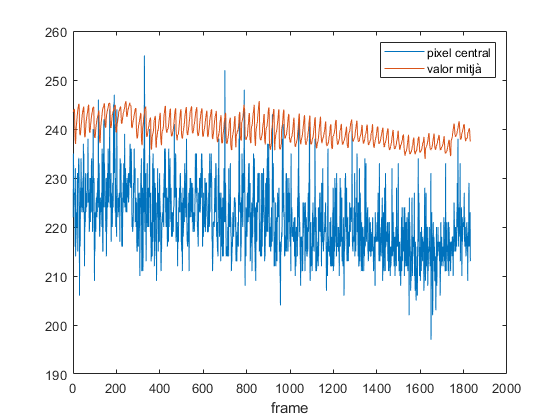
\includegraphics[width=0.35\textwidth]{fig2.png} 
\end{figure}

Ara sí que s'observa un comportament més senzill d'analitzar. Contem el nombre de períodes que hi ha en un interval de temps per obtenir un primer valor del pols i ens dóna 77 batecs/minut.

Per obtenir una mesura automàtica podem fer-ho de diverses maneres:
\begin{itemize}
\item trobar els creuaments del senyal quan talla el valor mitjà (en finestra lliscant)  i d'aquest temps deduir la freqüència (amb la inversa).
\item fer la transformada de Fourier d'una finestra de temps coneguda, obtenir el pic màxim que no estigui a prop de l'origen (primer harmònic) i deduir la freqüència a partir d'aquest valor. 
\end{itemize}
He optat pel segon mètode. A la figura veiem l'espectre de potència del senyal i el pic de l'harmònic principal. Amb aquest mètode també obtenim bons resultats amb el senyal sorollós de només un píxel.
\begin{figure}[h]
\centering
\begin{tabular}{cc}
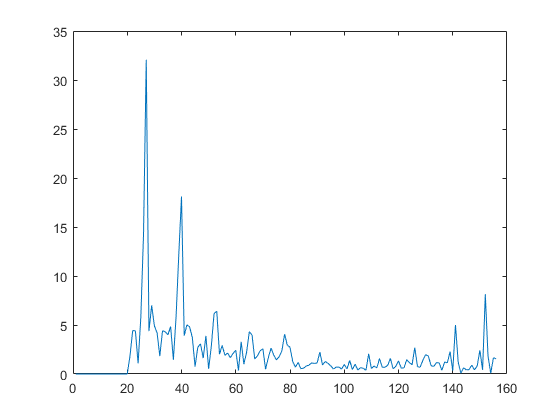
\includegraphics[width=0.2\textwidth]{fig3a.png} &
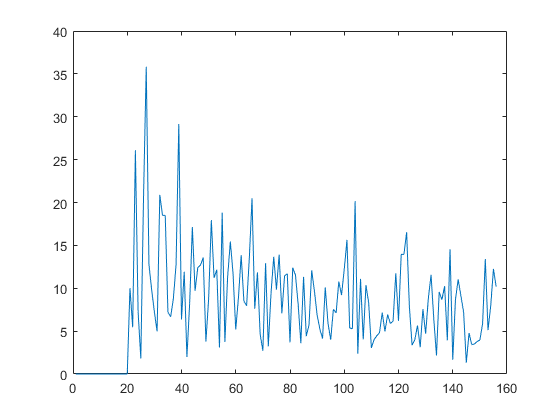
\includegraphics[width=0.2\textwidth]{fig3b.png} 
\end{tabular}
\end{figure}

El codi  de la solució final és aquest:

\begin{Verbatim}[fontsize=\small]
close all, clear global
v = VideoReader('.\VID_20210122_163105.mp4');
suau = [];
pix  = [];
frame = readFrame(v);
sz =size(frame);
while hasFrame(v)
  frame = readFrame(v);
  data = reshape(frame,sz(1)*sz(2),3);
  pix  = [pix data(sz(1)*sz(2)/2,1)]; %pixel mig R
  suau = [suau mean(data(:,1))]; %valor mitjà R
end
temps = v.Duration;
fprintf('temps: %f s\n',temps); % visualment 77 bat/min
figure, plot(pix')
hold on
plot(suau)

freq = abs(fft(suau));
freq(1:20)=0; %trec terme DC i primers valors
figure, plot(freq(1:end/2))
[~,pos] = max(freq(1:end/2));
fprintf('pols: %4.2f batecs/minut\n',60*pos/temps);

freq2 = abs(fft(pix));
freq2(1:20)=0; %trec terme DC i primers valors
figure, plot(freq2(1:end/2))
[~,pos] = max(freq2(1:end/2));
fprintf('pols: %4.2f batecs/minut\n',60*pos/temps);

>> pols: 76.60 batecs/minut
>> pols: 76.60 batecs/minut
\end{Verbatim}

\begin{thebibliography}{}
\item[$\diamond$] apunts de classe.
\end{thebibliography}		

\end{document}

